% !TEX TS-program = pdflatex
% !TEX encoding = UTF-8 Unicode

\documentclass[10pt,a4paper]{article}

\usepackage[utf8]{inputenc} % set input encoding to utf8


%%% PACKAGES
\usepackage{geometry}
\geometry{a4paper}
\usepackage{booktabs} % for much better looking tables
\usepackage{graphicx} % support the \includegraphics command and options
\usepackage{array} % for better arrays (eg matrices) in maths
\usepackage{paralist} % very flexible & customisable lists (eg. enumerate/itemize, etc.)
\usepackage{verbatim} % adds environment for commenting out blocks of text & for better verbatim
\usepackage[procnames]{listings} % for code segment environments.
% see http://en.wikibooks.org/wiki/LaTeX/Source_Code_Listings
\usepackage{tikz} % for FSM drawings from http://madebyevan.com/fsm/
\usepackage{qtree} % for \Tree
\usepackage{float} % unlocks [H] for float-placement.
\usepackage{subcaption} % unlocks the subfigure environment
\usepackage{multirow} % allows columns and rows to span multiple rows and colums, respectively
\usepackage{fancyhdr} % unlocks pagestyle 'fancy' and \[lcr](foot|head)
\usepackage{fullpage}
\usepackage{mathtools} % unlocks \DeclarePairedDelimiter
\usepackage{amsfonts} % unlocks \mathbb{}
\usepackage{color}
\usepackage{tgheros}

%\setcounter{secnumdepth}{3}

\DeclarePairedDelimiter{\ceil}{\lceil}{\rceil}
\DeclarePairedDelimiter{\floor}{\lfloor}{\rfloor}

\renewcommand\thesubsection{\alph{subsection})} % changes the subsection numbering to %LETTER%)
\renewcommand\thesubsubsection{\roman{subsubsection})} % changes the subsubsection numbering to %ROMAN%)
\renewcommand\thesection{Part \arabic{section}} % changes the section numbering to Part %NUMBER%

\usepackage[parfill]{parskip} % Activate to begin paragraphs with an empty line rather than an indent

\setlength{\headheight}{15pt} % distance between top of page and header
\setlength{\headsep}{30pt} %distance between the page text and header
\pagestyle{fancy}
%\renewcommand{\headrulewidth}{0pt}

\title{\reporttitle}
\author{\authorfull}
%\date{} % Delete this line to display the current date

\lhead{\coursefull}
\chead{}
\rhead{\texttt{\authorusrname}}





%%% BEGIN DOCUMENT
\begin{document}

\newpage
\maketitle
%\tableofcontents* % the asterisk means that the contents itself isn't put into the ToC


\section{Filtering}
\subsection{Something something discrete 1D convolutions}

\subsubsection{Compute some discrete convolution}
The given ``16 pixel wide image`` is actually 17 pixels wide.
$6+5+6 = 17$.
It's okay.
Don't sweat it.

Table~\ref{tab:11a} was produced using the partial filter method for the two first and last pixels in the image.

\begin{table}[H]
\centering
\begin{tabular}{|c|c|c|c|c|c|c|c|c|c|c|c|c|c|c|c|c|}
    \hline
    0 & 0 & 0 & 0 & 1 & 2 & 3 & 4 & 5 & 4 & 3 & 2 & 1 & 0 & 0 & 0 & 0 \\
    \hline
\end{tabular}
\caption{The discrete convolution of the given 5px wide filter and 17px wide image.}
\label{tab:11a}
\end{table}


\subsubsection{Do I see the need for any padding in the example?}
Nope!
If we pad the edges with zeroes the result is the same.
Padding with anything other than zeroes changes the result in a way that isn't representative of the original image with the given filter applied.

\subsection{Convolution}

\subsubsection{Compute the continuous convolution of two identical rectangular functions.}
The functions are $1$ in the range $[-\frac{1}{2}, \frac{1}{2}]$ and $0$ otherwise.

$$
(f * g)(t) =
\begin{cases}
    1+t & \text{if } -1 < t \leq 0 \\
    1-t & \text{if } 0 < t \leq 1 \\
    0 & \text{otherwise}
\end{cases}
$$

As $g$ slides along the axis from left to right it hits $f$ when $t=-1$.
For $t \in (-1, 0]$ the intersection of the areas of $f$ and $g$ grow from 0 to 1.
For $t \in (0, 1]$ the intersection decreases from 1 to 0.
The area of the intersection is 1 when $t$ is 0.

\subsubsection{What shape did I expect?}
It would make more sense to ask me this \textit{before} I computed the convolution.

But whatever: triangle!

\section{Spatial Filtering}

\subsection{Averaging Filter}
See Figure~\ref{fig:2-1-1} for the results from applying the averaging filter to the test image with salt \& pepper noise applied, and Figure~\ref{fig:2-1-2} for the ones for the test image with Gaussian noise applied to it.
The original noisy images are displayed for comparison.

\begin{figure}[h]
    \centering

    \begin{subfigure}[b]{0.3\textwidth}
        
\includegraphics[width=0.9\textwidth]{../code/2_out/2-1_sp.png}
        \caption{No filter.}
        \label{fig:2-1-1:1}
    \end{subfigure}
    \begin{subfigure}[b]{0.3\textwidth}
        
\includegraphics[width=0.9\textwidth]{../code/2_out/2-1_sp_3x3.png}
        \caption{3x3}
        \label{fig:2-1-1:2}
    \end{subfigure}

    \begin{subfigure}[b]{0.3\textwidth}
        
\includegraphics[width=0.9\textwidth]{../code/2_out/2-1_sp_5x5.png}
        \caption{5x5}
        \label{fig:2-1-1:3}
    \end{subfigure}
    \begin{subfigure}[b]{0.3\textwidth}
        
\includegraphics[width=0.9\textwidth]{../code/2_out/2-1_sp_9x9.png}
        \caption{9x9}
        \label{fig:2-1-1:4}
    \end{subfigure}

    \caption{Averaging filter of varying sizes applied to image with salt \& pepper noise.}
    \label{fig:2-1-1}
\end{figure}


\begin{figure}[h]
    \centering

    \begin{subfigure}[b]{0.3\textwidth}
        
\includegraphics[width=0.9\textwidth]{../code/2_out/2-1_gaus.png}
        \caption{No filter.}
        \label{fig:2-1-2:1}
    \end{subfigure}
    \begin{subfigure}[b]{0.3\textwidth}
        
\includegraphics[width=0.9\textwidth]{../code/2_out/2-1_gaus_3x3.png}
        \caption{3x3}
        \label{fig:2-1-2:2}
    \end{subfigure}

    \begin{subfigure}[b]{0.3\textwidth}
        
\includegraphics[width=0.9\textwidth]{../code/2_out/2-1_gaus_5x5.png}
        \caption{5x5}
        \label{fig:2-1-2:3}
    \end{subfigure}
    \begin{subfigure}[b]{0.3\textwidth}
        
\includegraphics[width=0.9\textwidth]{../code/2_out/2-1_gaus_9x9.png}
        \caption{9x9}
        \label{fig:2-1-2:4}
    \end{subfigure}

    \caption{Averaging filter of varying sizes applied to image with gaussian noise.}
    \label{fig:2-1-2}
\end{figure}

Code used to generate the images:
\inputminted[linenos=true]{octave}{../code/2.1.m}

\texttt{average.m}, the averaging filter function:
\inputminted[linenos=true]{octave}{../code/avgfilter.m}

\texttt{avg.m}, a function that computes the average (mean) value of a matrix:
\inputminted[linenos=true]{octave}{../code/avg.m}

\texttt{neighborhood.m}, a function that returns the \texttt{n x m} neighbourhood of a pixel at coordinates $(x,y)$ in a given image.
\inputminted[linenos=true]{octave}{../code/neighborhood.m}

\newpage

\section{Median Filtering}
We could probably compute the total difference in gray levels between the original and filtered images.
But I'm not sure if that's a useful metric or not.

Or we could create two new images showing the difference in gray level values between the original and filtered images.
But then again, judging the quality of the result of an image filter is highly subjective and depends on what one is looking for.

\begin{figure}[h]
    \centering

    \begin{subfigure}[b]{0.3\textwidth}
        
\includegraphics[width=0.9\textwidth]{../code/2_out/2-1_sp.png}
        \caption{No filter.}
        \label{fig:2-2-1:1}
    \end{subfigure}
    \begin{subfigure}[b]{0.3\textwidth}
        
\includegraphics[width=0.9\textwidth]{../code/2_out/2-2_sp_3x3.png}
        \caption{3x3}
        \label{fig:2-2-1:2}
    \end{subfigure}

    \begin{subfigure}[b]{0.3\textwidth}
        
\includegraphics[width=0.9\textwidth]{../code/2_out/2-2_sp_5x5.png}
        \caption{5x5}
        \label{fig:2-2-1:3}
    \end{subfigure}
    \begin{subfigure}[b]{0.3\textwidth}
        
\includegraphics[width=0.9\textwidth]{../code/2_out/2-2_sp_9x9.png}
        \caption{9x9}
        \label{fig:2-2-1:4}
    \end{subfigure}

    \caption{Median filter of varying sizes applied to image with salt \& pepper noise.}
    \label{fig:2-2-1}
\end{figure}


\begin{figure}[h]
    \centering

    \begin{subfigure}[b]{0.3\textwidth}
        
\includegraphics[width=0.9\textwidth]{../code/2_out/2-1_gaus.png}
        \caption{No filter.}
        \label{fig:2-2-2:1}
    \end{subfigure}
    \begin{subfigure}[b]{0.3\textwidth}
        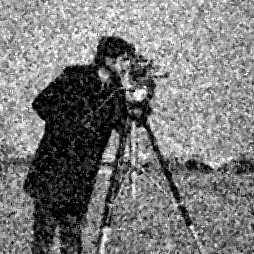
\includegraphics[width=0.9\textwidth]{../code/2_out/2-2_gaus_3x3.png}
        \caption{3x3}
        \label{fig:2-2-2:2}
    \end{subfigure}

    \begin{subfigure}[b]{0.3\textwidth}
        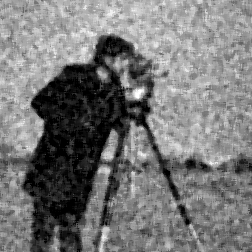
\includegraphics[width=0.9\textwidth]{../code/2_out/2-2_gaus_5x5.png}
        \caption{5x5}
        \label{fig:2-2-2:3}
    \end{subfigure}
    \begin{subfigure}[b]{0.3\textwidth}
        
\includegraphics[width=0.9\textwidth]{../code/2_out/2-2_gaus_9x9.png}
        \caption{9x9}
        \label{fig:2-2-2:4}
    \end{subfigure}

    \caption{Median filter of varying sizes applied to image with gaussian noise.}
    \label{fig:2-2-2}
\end{figure}

\newpage

\subsection{Anti-alias Filter}

Behold the answer in Figure~\ref{fig:2-3}.

\newcommand{\sftt}[1]{
    \begin{subfigure}[b]{0.3\textwidth}
        \includegraphics[width=0.9\textwidth]{../code/2_out/2-3_g#1.png}
        \caption{$\sigma = $#1}
        \label{fig:2-3:#1}
    \end{subfigure}
}

\begin{figure}[h]
\centering

    \begin{subfigure}[b]{0.3\textwidth}
        
\includegraphics[width=0.9\textwidth]{../code/img/lena.png}
        \caption{Original 512x512 image.}
        \label{fig:2-3:1}
    \end{subfigure}
    \begin{subfigure}[b]{0.3\textwidth}
        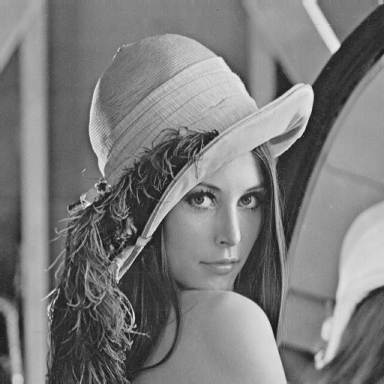
\includegraphics[width=0.9\textwidth]{../code/2_out/2-3_ds.png}
        \caption{3/4ths original size.}
        \label{fig:2-3:1}
    \end{subfigure}

    \sftt{0,5}
    \sftt{1}
    \sftt{2}

    \sftt{4}
    \sftt{8}
    \sftt{16}



\caption{Gaussian filter with varying sigmas applied to aliased image.}
\label{fig:2-3}
\end{figure}

Code used to generate images:
\inputminted[linenos=true]{octave}{../code/2.3.m}




\end{document}
